\newpage
\section{Problem 2: FREQUENCY DOMAIN}\label{problem-2-frequency-domain}
In this problem, please perform Fourier transform and observe the relation between the spatial domain and the frequency spectrum. You may adopt tools for Fourier transform. The recommended tools are listed in the Appendix.

Original image \nameref{sample2} for question \nameref{2_a} \nameref{2_b}, \nameref{2_c}.
\begin{figure}
    \centering
    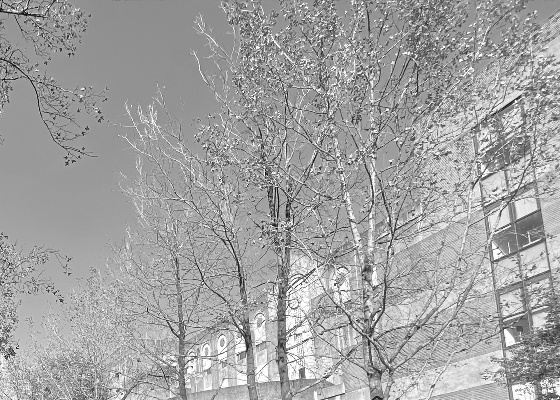
\includegraphics[width=0.7\textwidth]{src/sample2.png}
    \caption{\textbf{sample2.jpg}}
    \label{sample2}
\end{figure}

\subsection{(a)}\label{2_a}
Perform Fourier transform on \textbf{sample2.png} to obtain its frequency spectrum and output it as \textbf{result5.png}. (Please take the log magnitude of the absolute value and center the low frequency part at the origin for visualization.)

\paragraph{Motivation}

\paragraph{Approach}

\paragraph{Performance of results}
In the end, I choose the \alert{settings}...

Result of problem 2(a): \nameref{result5}.
\begin{figure}
    \centering
    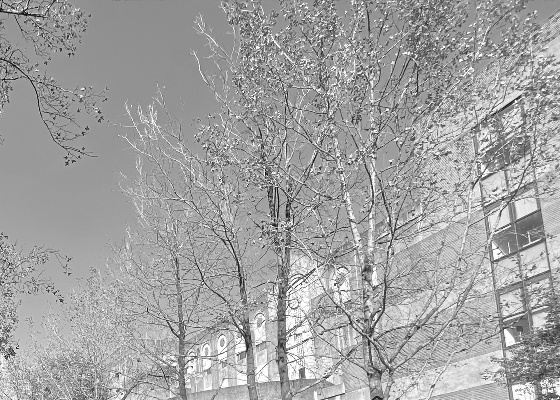
\includegraphics[width=0.7\textwidth]{src/sample2.png}
    \caption{\textbf{result5.jpg} Log axis of frequency domain}
    \label{result5}
\end{figure}

\paragraph{Discussion}

\subsection{(b)}\label{2_b}
Based on the result of part (a), design and apply a low-pass filter in the frequency domain and transform the result back to the pixel domain by inverse Fourier transform. The resultant image is saved as \textbf{result6.png}. Please also design a low-pass filter in the pixel domain which behaves similarly to the one you design in the frequency domain. Output the result as \textbf{result7.png} and provide some discussions.

\paragraph{Motivation}

\paragraph{Approach}

\paragraph{Performance of results}
In the end, I choose the \alert{settings}...

Result of problem 2(b): \nameref{result6}.
\begin{figure}
    \centering
    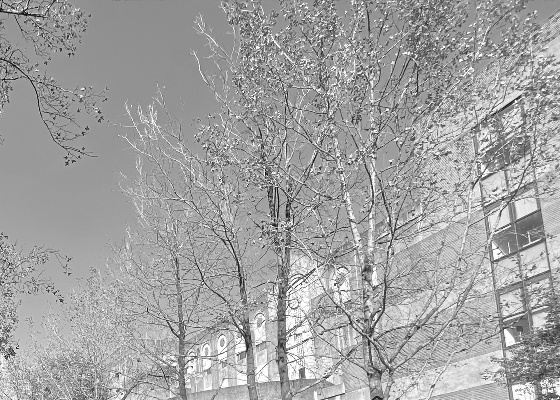
\includegraphics[width=0.7\textwidth]{src/sample2.png}
    \caption{\textbf{result6.jpg} Low-pass filter in frequency domain}
    \label{result6}
\end{figure}

Result of problem 2(b): \nameref{result7}.
\begin{figure}
    \centering
    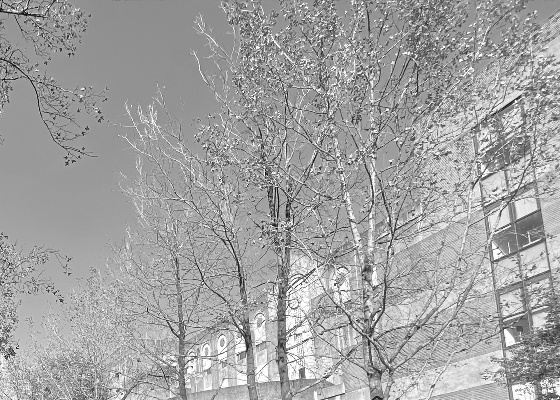
\includegraphics[width=0.7\textwidth]{src/sample2.png}
    \caption{\textbf{result7.jpg} Low-pass filter in spatial domain}
    \label{result7}
\end{figure}

\paragraph{Discussion}
Compare \nameref{result6} with \nameref{result7}.

\subsection{(c)}\label{2_c}
Based on the result of part (a), design and apply a high-pass filter in the frequency domain and transform the result back to the pixel domain by inverse Fourier transform. The resultant image is saved as \textbf{result8.png}. Please also design a high-pass filter in the pixel domain which behaves similarly to the one you design in the frequency domain. Output the result as \textbf{result9.png} and provide some discussions.

\paragraph{Motivation}

\paragraph{Approach}

\paragraph{Performance of results}
In the end, I choose the \alert{settings}...

Result of problem 2(c): \nameref{result8}.
\begin{figure}
    \centering
    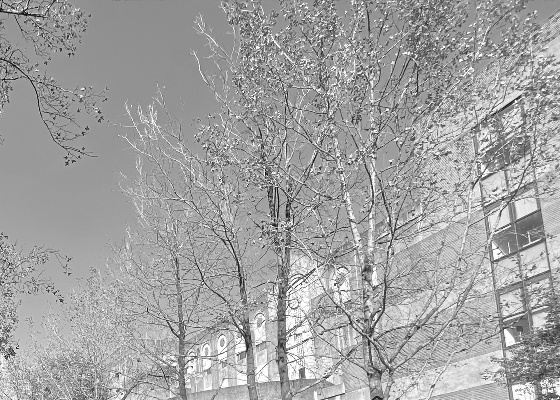
\includegraphics[width=0.7\textwidth]{src/sample2.png}
    \caption{\textbf{result8.jpg} High-pass filter in frequency domain}
    \label{result8}
\end{figure}

Result of problem 2(c): \nameref{result9}.
\begin{figure}
    \centering
    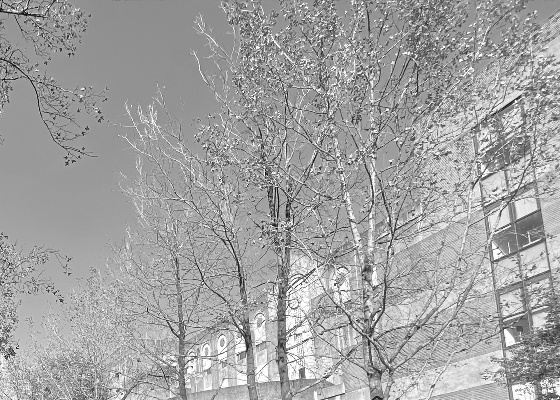
\includegraphics[width=0.7\textwidth]{src/sample2.png}
    \caption{\textbf{result7.jpg} High-pass filter in spatial domain}
    \label{result9}
\end{figure}

\paragraph{Discussion}
Compare \nameref{result8} with \nameref{result9}.

Original image \nameref{sample3} for question \nameref{2_d} \nameref{2_e}.
\begin{figure}
    \centering
    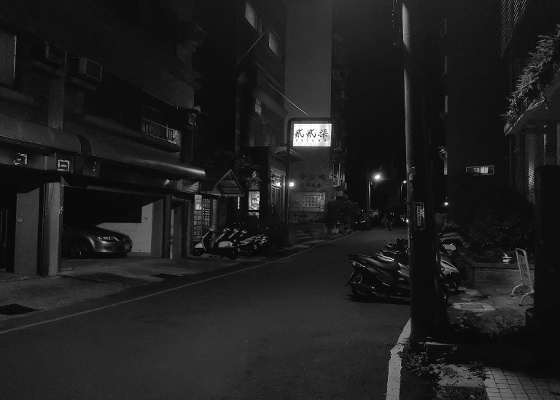
\includegraphics[width=0.7\textwidth]{src/sample3.png}
    \caption{\textbf{sample3.jpg}}
    \label{sample3}
\end{figure}

\subsection{(d)}\label{2_d}
Perform Fourier Transform on \textbf{sample3.png} and output it as \textbf{result10.png}. Please discuss what you observe in \textbf{sample3.png} and \textbf{result10.png}.

\paragraph{Motivation}

\paragraph{Approach}

\paragraph{Performance of results}
In the end, I choose the \alert{settings}...

Result of problem 2(d): \nameref{result10}.
\begin{figure}
    \centering
    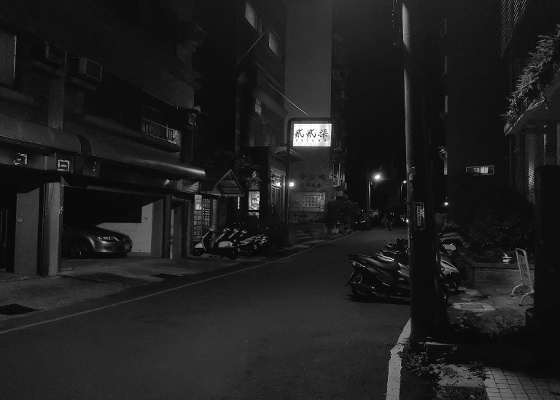
\includegraphics[width=0.7\textwidth]{src/sample3.png}
    \caption{\textbf{result10.jpg} Fourier Transform on \nameref{sample3}}
    \label{result10}
\end{figure}

\paragraph{Discussion}
Observe in \nameref{sample3} and \nameref{result10}.

\subsection{(e)}\label{2_e}
Try to remove the undesired pattern on \textbf{sample3.png} and output it as \textbf{result11.png}.

\paragraph{Motivation}

\paragraph{Approach}

\paragraph{Performance of results}
In the end, I choose the \alert{settings}...

Result of problem 2(e): \nameref{result11}.
\begin{figure}
    \centering
    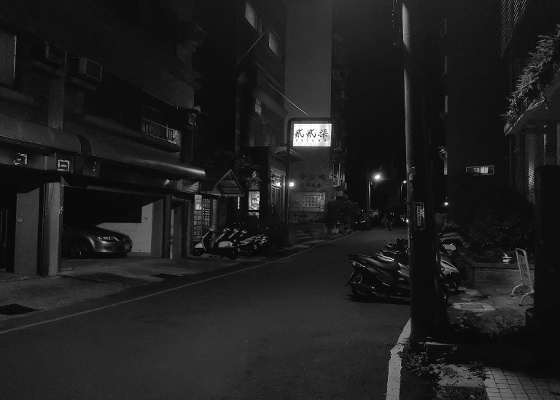
\includegraphics[width=0.7\textwidth]{src/sample3.png}
    \caption{\textbf{result11.jpg} Noise cleaning of \nameref{sample3}}
    \label{result11}
\end{figure}

\paragraph{Discussion}
